
% Default to the notebook output style

    


% Inherit from the specified cell style.




    
\documentclass[11pt]{article}

    
    
    \usepackage[T1]{fontenc}
    % Nicer default font (+ math font) than Computer Modern for most use cases
    \usepackage{mathpazo}
	\usepackage{float}
    % Basic figure setup, for now with no caption control since it's done
    % automatically by Pandoc (which extracts ![](path) syntax from Markdown).
    \usepackage{graphicx}
    % We will generate all images so they have a width \maxwidth. This means
    % that they will get their normal width if they fit onto the page, but
    % are scaled down if they would overflow the margins.
    \makeatletter
    \def\maxwidth{\ifdim\Gin@nat@width>\linewidth\linewidth
    \else\Gin@nat@width\fi}
    \makeatother
    \let\Oldincludegraphics\includegraphics
    % Set max figure width to be 80% of text width, for now hardcoded.
    \renewcommand{\includegraphics}[1]{\Oldincludegraphics[width=.8\maxwidth]{#1}}
    % Ensure that by default, figures have no caption (until we provide a
    % proper Figure object with a Caption API and a way to capture that
    % in the conversion process - todo).
    \usepackage{caption}
    \DeclareCaptionLabelFormat{nolabel}{}
    \captionsetup{labelformat=nolabel}

    \usepackage{adjustbox} % Used to constrain images to a maximum size 
    \usepackage{xcolor} % Allow colors to be defined
    \usepackage{enumerate} % Needed for markdown enumerations to work
    \usepackage{geometry} % Used to adjust the document margins
    \usepackage{amsmath} % Equations
    \usepackage{amssymb} % Equations
    \usepackage{textcomp} % defines textquotesingle
    % Hack from http://tex.stackexchange.com/a/47451/13684:
    \AtBeginDocument{%
        \def\PYZsq{\textquotesingle}% Upright quotes in Pygmentized code
    }
    \usepackage{upquote} % Upright quotes for verbatim code
    \usepackage{eurosym} % defines \euro
    \usepackage[mathletters]{ucs} % Extended unicode (utf-8) support
    \usepackage[utf8x]{inputenc} % Allow utf-8 characters in the tex document
    \usepackage{fancyvrb} % verbatim replacement that allows latex
    \usepackage{grffile} % extends the file name processing of package graphics 
                         % to support a larger range 
    % The hyperref package gives us a pdf with properly built
    % internal navigation ('pdf bookmarks' for the table of contents,
    % internal cross-reference links, web links for URLs, etc.)
    \usepackage{hyperref}
    \usepackage{longtable} % longtable support required by pandoc >1.10
    \usepackage{booktabs}  % table support for pandoc > 1.12.2
    \usepackage[inline]{enumitem} % IRkernel/repr support (it uses the enumerate* environment)
    \usepackage[normalem]{ulem} % ulem is needed to support strikethroughs (\sout)
                                % normalem makes italics be italics, not underlines
    \usepackage{mathrsfs}
    

    
    
    % Colors for the hyperref package
    \definecolor{urlcolor}{rgb}{0,.145,.698}
    \definecolor{linkcolor}{rgb}{.71,0.21,0.01}
    \definecolor{citecolor}{rgb}{.12,.54,.11}

    % ANSI colors
    \definecolor{ansi-black}{HTML}{3E424D}
    \definecolor{ansi-black-intense}{HTML}{282C36}
    \definecolor{ansi-red}{HTML}{E75C58}
    \definecolor{ansi-red-intense}{HTML}{B22B31}
    \definecolor{ansi-green}{HTML}{00A250}
    \definecolor{ansi-green-intense}{HTML}{007427}
    \definecolor{ansi-yellow}{HTML}{DDB62B}
    \definecolor{ansi-yellow-intense}{HTML}{B27D12}
    \definecolor{ansi-blue}{HTML}{208FFB}
    \definecolor{ansi-blue-intense}{HTML}{0065CA}
    \definecolor{ansi-magenta}{HTML}{D160C4}
    \definecolor{ansi-magenta-intense}{HTML}{A03196}
    \definecolor{ansi-cyan}{HTML}{60C6C8}
    \definecolor{ansi-cyan-intense}{HTML}{258F8F}
    \definecolor{ansi-white}{HTML}{C5C1B4}
    \definecolor{ansi-white-intense}{HTML}{A1A6B2}
    \definecolor{ansi-default-inverse-fg}{HTML}{FFFFFF}
    \definecolor{ansi-default-inverse-bg}{HTML}{000000}

    % commands and environments needed by pandoc snippets
    % extracted from the output of `pandoc -s`
    \providecommand{\tightlist}{%
      \setlength{\itemsep}{0pt}\setlength{\parskip}{0pt}}
    \DefineVerbatimEnvironment{Highlighting}{Verbatim}{commandchars=\\\{\}}
    % Add ',fontsize=\small' for more characters per line
    \newenvironment{Shaded}{}{}
    \newcommand{\KeywordTok}[1]{\textcolor[rgb]{0.00,0.44,0.13}{\textbf{{#1}}}}
    \newcommand{\DataTypeTok}[1]{\textcolor[rgb]{0.56,0.13,0.00}{{#1}}}
    \newcommand{\DecValTok}[1]{\textcolor[rgb]{0.25,0.63,0.44}{{#1}}}
    \newcommand{\BaseNTok}[1]{\textcolor[rgb]{0.25,0.63,0.44}{{#1}}}
    \newcommand{\FloatTok}[1]{\textcolor[rgb]{0.25,0.63,0.44}{{#1}}}
    \newcommand{\CharTok}[1]{\textcolor[rgb]{0.25,0.44,0.63}{{#1}}}
    \newcommand{\StringTok}[1]{\textcolor[rgb]{0.25,0.44,0.63}{{#1}}}
    \newcommand{\CommentTok}[1]{\textcolor[rgb]{0.38,0.63,0.69}{\textit{{#1}}}}
    \newcommand{\OtherTok}[1]{\textcolor[rgb]{0.00,0.44,0.13}{{#1}}}
    \newcommand{\AlertTok}[1]{\textcolor[rgb]{1.00,0.00,0.00}{\textbf{{#1}}}}
    \newcommand{\FunctionTok}[1]{\textcolor[rgb]{0.02,0.16,0.49}{{#1}}}
    \newcommand{\RegionMarkerTok}[1]{{#1}}
    \newcommand{\ErrorTok}[1]{\textcolor[rgb]{1.00,0.00,0.00}{\textbf{{#1}}}}
    \newcommand{\NormalTok}[1]{{#1}}
    
    % Additional commands for more recent versions of Pandoc
    \newcommand{\ConstantTok}[1]{\textcolor[rgb]{0.53,0.00,0.00}{{#1}}}
    \newcommand{\SpecialCharTok}[1]{\textcolor[rgb]{0.25,0.44,0.63}{{#1}}}
    \newcommand{\VerbatimStringTok}[1]{\textcolor[rgb]{0.25,0.44,0.63}{{#1}}}
    \newcommand{\SpecialStringTok}[1]{\textcolor[rgb]{0.73,0.40,0.53}{{#1}}}
    \newcommand{\ImportTok}[1]{{#1}}
    \newcommand{\DocumentationTok}[1]{\textcolor[rgb]{0.73,0.13,0.13}{\textit{{#1}}}}
    \newcommand{\AnnotationTok}[1]{\textcolor[rgb]{0.38,0.63,0.69}{\textbf{\textit{{#1}}}}}
    \newcommand{\CommentVarTok}[1]{\textcolor[rgb]{0.38,0.63,0.69}{\textbf{\textit{{#1}}}}}
    \newcommand{\VariableTok}[1]{\textcolor[rgb]{0.10,0.09,0.49}{{#1}}}
    \newcommand{\ControlFlowTok}[1]{\textcolor[rgb]{0.00,0.44,0.13}{\textbf{{#1}}}}
    \newcommand{\OperatorTok}[1]{\textcolor[rgb]{0.40,0.40,0.40}{{#1}}}
    \newcommand{\BuiltInTok}[1]{{#1}}
    \newcommand{\ExtensionTok}[1]{{#1}}
    \newcommand{\PreprocessorTok}[1]{\textcolor[rgb]{0.74,0.48,0.00}{{#1}}}
    \newcommand{\AttributeTok}[1]{\textcolor[rgb]{0.49,0.56,0.16}{{#1}}}
    \newcommand{\InformationTok}[1]{\textcolor[rgb]{0.38,0.63,0.69}{\textbf{\textit{{#1}}}}}
    \newcommand{\WarningTok}[1]{\textcolor[rgb]{0.38,0.63,0.69}{\textbf{\textit{{#1}}}}}
    
    
    % Define a nice break command that doesn't care if a line doesn't already
    % exist.
    \def\br{\hspace*{\fill} \\* }
    % Math Jax compatibility definitions
    \def\gt{>}
    \def\lt{<}
    \let\Oldtex\TeX
    \let\Oldlatex\LaTeX
    \renewcommand{\TeX}{\textrm{\Oldtex}}
    \renewcommand{\LaTeX}{\textrm{\Oldlatex}}
    % Document parameters
    % Document title
    \title{Assignment 4}
    
    
    \author{Jiarong Ye}
    
    

    % Pygments definitions
    
\makeatletter
\def\PY@reset{\let\PY@it=\relax \let\PY@bf=\relax%
    \let\PY@ul=\relax \let\PY@tc=\relax%
    \let\PY@bc=\relax \let\PY@ff=\relax}
\def\PY@tok#1{\csname PY@tok@#1\endcsname}
\def\PY@toks#1+{\ifx\relax#1\empty\else%
    \PY@tok{#1}\expandafter\PY@toks\fi}
\def\PY@do#1{\PY@bc{\PY@tc{\PY@ul{%
    \PY@it{\PY@bf{\PY@ff{#1}}}}}}}
\def\PY#1#2{\PY@reset\PY@toks#1+\relax+\PY@do{#2}}

\expandafter\def\csname PY@tok@w\endcsname{\def\PY@tc##1{\textcolor[rgb]{0.73,0.73,0.73}{##1}}}
\expandafter\def\csname PY@tok@c\endcsname{\let\PY@it=\textit\def\PY@tc##1{\textcolor[rgb]{0.25,0.50,0.50}{##1}}}
\expandafter\def\csname PY@tok@cp\endcsname{\def\PY@tc##1{\textcolor[rgb]{0.74,0.48,0.00}{##1}}}
\expandafter\def\csname PY@tok@k\endcsname{\let\PY@bf=\textbf\def\PY@tc##1{\textcolor[rgb]{0.00,0.50,0.00}{##1}}}
\expandafter\def\csname PY@tok@kp\endcsname{\def\PY@tc##1{\textcolor[rgb]{0.00,0.50,0.00}{##1}}}
\expandafter\def\csname PY@tok@kt\endcsname{\def\PY@tc##1{\textcolor[rgb]{0.69,0.00,0.25}{##1}}}
\expandafter\def\csname PY@tok@o\endcsname{\def\PY@tc##1{\textcolor[rgb]{0.40,0.40,0.40}{##1}}}
\expandafter\def\csname PY@tok@ow\endcsname{\let\PY@bf=\textbf\def\PY@tc##1{\textcolor[rgb]{0.67,0.13,1.00}{##1}}}
\expandafter\def\csname PY@tok@nb\endcsname{\def\PY@tc##1{\textcolor[rgb]{0.00,0.50,0.00}{##1}}}
\expandafter\def\csname PY@tok@nf\endcsname{\def\PY@tc##1{\textcolor[rgb]{0.00,0.00,1.00}{##1}}}
\expandafter\def\csname PY@tok@nc\endcsname{\let\PY@bf=\textbf\def\PY@tc##1{\textcolor[rgb]{0.00,0.00,1.00}{##1}}}
\expandafter\def\csname PY@tok@nn\endcsname{\let\PY@bf=\textbf\def\PY@tc##1{\textcolor[rgb]{0.00,0.00,1.00}{##1}}}
\expandafter\def\csname PY@tok@ne\endcsname{\let\PY@bf=\textbf\def\PY@tc##1{\textcolor[rgb]{0.82,0.25,0.23}{##1}}}
\expandafter\def\csname PY@tok@nv\endcsname{\def\PY@tc##1{\textcolor[rgb]{0.10,0.09,0.49}{##1}}}
\expandafter\def\csname PY@tok@no\endcsname{\def\PY@tc##1{\textcolor[rgb]{0.53,0.00,0.00}{##1}}}
\expandafter\def\csname PY@tok@nl\endcsname{\def\PY@tc##1{\textcolor[rgb]{0.63,0.63,0.00}{##1}}}
\expandafter\def\csname PY@tok@ni\endcsname{\let\PY@bf=\textbf\def\PY@tc##1{\textcolor[rgb]{0.60,0.60,0.60}{##1}}}
\expandafter\def\csname PY@tok@na\endcsname{\def\PY@tc##1{\textcolor[rgb]{0.49,0.56,0.16}{##1}}}
\expandafter\def\csname PY@tok@nt\endcsname{\let\PY@bf=\textbf\def\PY@tc##1{\textcolor[rgb]{0.00,0.50,0.00}{##1}}}
\expandafter\def\csname PY@tok@nd\endcsname{\def\PY@tc##1{\textcolor[rgb]{0.67,0.13,1.00}{##1}}}
\expandafter\def\csname PY@tok@s\endcsname{\def\PY@tc##1{\textcolor[rgb]{0.73,0.13,0.13}{##1}}}
\expandafter\def\csname PY@tok@sd\endcsname{\let\PY@it=\textit\def\PY@tc##1{\textcolor[rgb]{0.73,0.13,0.13}{##1}}}
\expandafter\def\csname PY@tok@si\endcsname{\let\PY@bf=\textbf\def\PY@tc##1{\textcolor[rgb]{0.73,0.40,0.53}{##1}}}
\expandafter\def\csname PY@tok@se\endcsname{\let\PY@bf=\textbf\def\PY@tc##1{\textcolor[rgb]{0.73,0.40,0.13}{##1}}}
\expandafter\def\csname PY@tok@sr\endcsname{\def\PY@tc##1{\textcolor[rgb]{0.73,0.40,0.53}{##1}}}
\expandafter\def\csname PY@tok@ss\endcsname{\def\PY@tc##1{\textcolor[rgb]{0.10,0.09,0.49}{##1}}}
\expandafter\def\csname PY@tok@sx\endcsname{\def\PY@tc##1{\textcolor[rgb]{0.00,0.50,0.00}{##1}}}
\expandafter\def\csname PY@tok@m\endcsname{\def\PY@tc##1{\textcolor[rgb]{0.40,0.40,0.40}{##1}}}
\expandafter\def\csname PY@tok@gh\endcsname{\let\PY@bf=\textbf\def\PY@tc##1{\textcolor[rgb]{0.00,0.00,0.50}{##1}}}
\expandafter\def\csname PY@tok@gu\endcsname{\let\PY@bf=\textbf\def\PY@tc##1{\textcolor[rgb]{0.50,0.00,0.50}{##1}}}
\expandafter\def\csname PY@tok@gd\endcsname{\def\PY@tc##1{\textcolor[rgb]{0.63,0.00,0.00}{##1}}}
\expandafter\def\csname PY@tok@gi\endcsname{\def\PY@tc##1{\textcolor[rgb]{0.00,0.63,0.00}{##1}}}
\expandafter\def\csname PY@tok@gr\endcsname{\def\PY@tc##1{\textcolor[rgb]{1.00,0.00,0.00}{##1}}}
\expandafter\def\csname PY@tok@ge\endcsname{\let\PY@it=\textit}
\expandafter\def\csname PY@tok@gs\endcsname{\let\PY@bf=\textbf}
\expandafter\def\csname PY@tok@gp\endcsname{\let\PY@bf=\textbf\def\PY@tc##1{\textcolor[rgb]{0.00,0.00,0.50}{##1}}}
\expandafter\def\csname PY@tok@go\endcsname{\def\PY@tc##1{\textcolor[rgb]{0.53,0.53,0.53}{##1}}}
\expandafter\def\csname PY@tok@gt\endcsname{\def\PY@tc##1{\textcolor[rgb]{0.00,0.27,0.87}{##1}}}
\expandafter\def\csname PY@tok@err\endcsname{\def\PY@bc##1{\setlength{\fboxsep}{0pt}\fcolorbox[rgb]{1.00,0.00,0.00}{1,1,1}{\strut ##1}}}
\expandafter\def\csname PY@tok@kc\endcsname{\let\PY@bf=\textbf\def\PY@tc##1{\textcolor[rgb]{0.00,0.50,0.00}{##1}}}
\expandafter\def\csname PY@tok@kd\endcsname{\let\PY@bf=\textbf\def\PY@tc##1{\textcolor[rgb]{0.00,0.50,0.00}{##1}}}
\expandafter\def\csname PY@tok@kn\endcsname{\let\PY@bf=\textbf\def\PY@tc##1{\textcolor[rgb]{0.00,0.50,0.00}{##1}}}
\expandafter\def\csname PY@tok@kr\endcsname{\let\PY@bf=\textbf\def\PY@tc##1{\textcolor[rgb]{0.00,0.50,0.00}{##1}}}
\expandafter\def\csname PY@tok@bp\endcsname{\def\PY@tc##1{\textcolor[rgb]{0.00,0.50,0.00}{##1}}}
\expandafter\def\csname PY@tok@fm\endcsname{\def\PY@tc##1{\textcolor[rgb]{0.00,0.00,1.00}{##1}}}
\expandafter\def\csname PY@tok@vc\endcsname{\def\PY@tc##1{\textcolor[rgb]{0.10,0.09,0.49}{##1}}}
\expandafter\def\csname PY@tok@vg\endcsname{\def\PY@tc##1{\textcolor[rgb]{0.10,0.09,0.49}{##1}}}
\expandafter\def\csname PY@tok@vi\endcsname{\def\PY@tc##1{\textcolor[rgb]{0.10,0.09,0.49}{##1}}}
\expandafter\def\csname PY@tok@vm\endcsname{\def\PY@tc##1{\textcolor[rgb]{0.10,0.09,0.49}{##1}}}
\expandafter\def\csname PY@tok@sa\endcsname{\def\PY@tc##1{\textcolor[rgb]{0.73,0.13,0.13}{##1}}}
\expandafter\def\csname PY@tok@sb\endcsname{\def\PY@tc##1{\textcolor[rgb]{0.73,0.13,0.13}{##1}}}
\expandafter\def\csname PY@tok@sc\endcsname{\def\PY@tc##1{\textcolor[rgb]{0.73,0.13,0.13}{##1}}}
\expandafter\def\csname PY@tok@dl\endcsname{\def\PY@tc##1{\textcolor[rgb]{0.73,0.13,0.13}{##1}}}
\expandafter\def\csname PY@tok@s2\endcsname{\def\PY@tc##1{\textcolor[rgb]{0.73,0.13,0.13}{##1}}}
\expandafter\def\csname PY@tok@sh\endcsname{\def\PY@tc##1{\textcolor[rgb]{0.73,0.13,0.13}{##1}}}
\expandafter\def\csname PY@tok@s1\endcsname{\def\PY@tc##1{\textcolor[rgb]{0.73,0.13,0.13}{##1}}}
\expandafter\def\csname PY@tok@mb\endcsname{\def\PY@tc##1{\textcolor[rgb]{0.40,0.40,0.40}{##1}}}
\expandafter\def\csname PY@tok@mf\endcsname{\def\PY@tc##1{\textcolor[rgb]{0.40,0.40,0.40}{##1}}}
\expandafter\def\csname PY@tok@mh\endcsname{\def\PY@tc##1{\textcolor[rgb]{0.40,0.40,0.40}{##1}}}
\expandafter\def\csname PY@tok@mi\endcsname{\def\PY@tc##1{\textcolor[rgb]{0.40,0.40,0.40}{##1}}}
\expandafter\def\csname PY@tok@il\endcsname{\def\PY@tc##1{\textcolor[rgb]{0.40,0.40,0.40}{##1}}}
\expandafter\def\csname PY@tok@mo\endcsname{\def\PY@tc##1{\textcolor[rgb]{0.40,0.40,0.40}{##1}}}
\expandafter\def\csname PY@tok@ch\endcsname{\let\PY@it=\textit\def\PY@tc##1{\textcolor[rgb]{0.25,0.50,0.50}{##1}}}
\expandafter\def\csname PY@tok@cm\endcsname{\let\PY@it=\textit\def\PY@tc##1{\textcolor[rgb]{0.25,0.50,0.50}{##1}}}
\expandafter\def\csname PY@tok@cpf\endcsname{\let\PY@it=\textit\def\PY@tc##1{\textcolor[rgb]{0.25,0.50,0.50}{##1}}}
\expandafter\def\csname PY@tok@c1\endcsname{\let\PY@it=\textit\def\PY@tc##1{\textcolor[rgb]{0.25,0.50,0.50}{##1}}}
\expandafter\def\csname PY@tok@cs\endcsname{\let\PY@it=\textit\def\PY@tc##1{\textcolor[rgb]{0.25,0.50,0.50}{##1}}}

\def\PYZbs{\char`\\}
\def\PYZus{\char`\_}
\def\PYZob{\char`\{}
\def\PYZcb{\char`\}}
\def\PYZca{\char`\^}
\def\PYZam{\char`\&}
\def\PYZlt{\char`\<}
\def\PYZgt{\char`\>}
\def\PYZsh{\char`\#}
\def\PYZpc{\char`\%}
\def\PYZdl{\char`\$}
\def\PYZhy{\char`\-}
\def\PYZsq{\char`\'}
\def\PYZdq{\char`\"}
\def\PYZti{\char`\~}
% for compatibility with earlier versions
\def\PYZat{@}
\def\PYZlb{[}
\def\PYZrb{]}
\makeatother


    % Exact colors from NB
    \definecolor{incolor}{rgb}{0.0, 0.0, 0.5}
    \definecolor{outcolor}{rgb}{0.545, 0.0, 0.0}



    
    % Prevent overflowing lines due to hard-to-break entities
    \sloppy 
    % Setup hyperref package
    \hypersetup{
      breaklinks=true,  % so long urls are correctly broken across lines
      colorlinks=true,
      urlcolor=urlcolor,
      linkcolor=linkcolor,
      citecolor=citecolor,
      }
    % Slightly bigger margins than the latex defaults
    
    \geometry{verbose,tmargin=1in,bmargin=1in,lmargin=1in,rmargin=1in}
    
    

    \begin{document}
    
    
    \maketitle
    
    


    \subsubsection*{Q1}\label{q1}

    Consider a completely randomized design with observations on three
treatments coded 1,2,3. For the one-way ANOVA model, determine which of
the following are estimable. For those that are estimable, write out the
estimable function as \(\sum^3_i=b_i(\mu + \tau_i)\) and clearly state
\(b_1, b_2, b_3\). Finally, for those that are estimable, state the
least squares estimator.

    \begin{itemize}
\item
  \begin{enumerate}
  \def\labelenumi{\alph{enumi})}
  \tightlist
  \item
    \(\tau_1+ \tau_2 - 2\tau_3\)
  \end{enumerate}
\end{itemize}

Suppose it is estimable, then it should be represented as

\[\tau_1+ \tau_2 - 2\tau_3 = b_1 (\mu + \tau_1) + b_2 (\mu + \tau_2) + b_3 (\mu + \tau_3)\]

\[= \mu (b_1+b_2+b_3) + b_1 \tau_1 + b_2 \tau_2 + b_3 \tau_3\]

\begin{align}
\left\{\begin{matrix} (b_1+b_2+b_3) =0
\\ b_1 = 1
\\ b_2 = 1
\\ b_3 = -2
\end{matrix}\right.
\end{align}

Therefore,
\(\tau_1+ \tau_2 - 2\tau_3 = 1 \cdot (\mu + \tau_1) + 1 \cdot (\mu + \tau_2) + (-2) \cdot (\mu + \tau_3)\),
it is estimable.



\begin{itemize}
\item
  \begin{enumerate}
  \def\labelenumi{\alph{enumi})}
  \setcounter{enumi}{1}
  \tightlist
  \item
    \(\mu + \tau_3\)
  \end{enumerate}
\end{itemize}

Suppose it is estimable, then it should be represented as

\[\mu + \tau_3 = b_1 (\mu + \tau_1) + b_2 (\mu + \tau_2) + b_3 (\mu + \tau_3)\]

\[= \mu (b_1+b_2+b_3) + b_1 \tau_1 + b_2 \tau_2 + b_3 \tau_3\]

\begin{align}
\left\{\begin{matrix} (b_1+b_2+b_3) =1
\\ b_1 = 0
\\ b_2 = 0
\\ b_3 = 1
\end{matrix}\right.
\end{align}

Therefore,
\(\mu + \tau_3 = 0 \cdot (\mu + \tau_1) + 0 \cdot (\mu + \tau_2) + 1 \cdot (\mu + \tau_3)\)
, it is estimable.



\begin{itemize}
\item
  \begin{enumerate}
  \def\labelenumi{\alph{enumi})}
  \setcounter{enumi}{2}
  \tightlist
  \item
    \(\tau_1-\tau_2-\tau_3\)
  \end{enumerate}
\end{itemize}

Suppose it is estimable, then it should be represented as

\[\tau_1-\tau_2-\tau_3 = b_1 (\mu + \tau_1) + b_2 (\mu + \tau_2) + b_3 (\mu + \tau_3)\]

\[= \mu (b_1+b_2+b_3) + b_1 \tau_1 + b_2 \tau_2 + b_3 \tau_3\]

\begin{align}
\left\{\begin{matrix} (b_1+b_2+b_3) =0
\\ b_1 = 1
\\ b_2 = -1
\\ b_3 = -1
\end{matrix}\right.
\end{align}

And here, if \(b_1 = 1, b_2 = -1, b_3 = -1\), then
\(b_1+b_2+b_3 = -1 \neq 0\), it contradicts with  \( (b_1+b_2+b_3)
=0\)

Therefore, \(\tau_1-\tau_2-\tau_3\) is not estimable.



\begin{itemize}
\item
  \begin{enumerate}
  \def\labelenumi{\alph{enumi})}
  \setcounter{enumi}{3}
  \tightlist
  \item
    \(\mu + (\tau_1 + \tau_2 + \tau_3) /3\)
  \end{enumerate}
\end{itemize}

Suppose it is estimable, then it should be represented as

\[\mu + (\tau_1 + \tau_2 + \tau_3) /3 = b_1 (\mu + \tau_1) + b_2 (\mu + \tau_2) + b_3 (\mu + \tau_3)\]

\[= \mu (b_1+b_2+b_3) + b_1 \tau_1 + b_2 \tau_2 + b_3 \tau_3\]

\begin{align}
\left\{\begin{matrix} (b_1+b_2+b_3) =1
\\ b_1 = \frac{1}{3}
\\ b_2 = \frac{1}{3}
\\ b_3 = \frac{1}{3}
\end{matrix}\right.
\end{align}

Therefore,
\(\mu + (\tau_1 + \tau_2 + \tau_3) /3 = \frac{1}{3} \cdot (\mu + \tau_1) + \frac{1}{3} \cdot (\mu + \tau_2) + \frac{1}{3} \cdot (\mu + \tau_3)\)
, it is estimable.

    \subsubsection*{Q2}\label{q2}

    Recall the soap experiment from Homework 1. Look back at Homework 1 for
an explanation of the experiment. The data are the weight lost over 24
hours by different types of soap.

\begin{figure}[H]
\centering
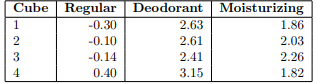
\includegraphics{table.png}
\caption{}
\end{figure}

    \begin{itemize}
\item
  \begin{enumerate}
  \def\labelenumi{(\alph{enumi})}
  \tightlist
  \item
    Write out the one-way ANOVA model for this experiment.
  \end{enumerate}
\end{itemize}

    \begin{Verbatim}[commandchars=\\\{\}]
{\color{incolor}In [{\color{incolor}11}]:} \PY{k+kn}{library}\PY{p}{(}lsmeans\PY{p}{)}
         types \PY{o}{=} \PY{k+kt}{c}\PY{p}{(}\PY{l+s}{\PYZsq{}}\PY{l+s}{Regular\PYZsq{}}\PY{p}{,} \PY{l+s}{\PYZsq{}}\PY{l+s}{Deodorant\PYZsq{}}\PY{p}{,} \PY{l+s}{\PYZsq{}}\PY{l+s}{Moisturizing\PYZsq{}}\PY{p}{)}
         soap\PYZus{}type \PY{o}{=} \PY{k+kt}{c}\PY{p}{(}\PY{k+kp}{rep}\PY{p}{(}types\PY{p}{[}\PY{l+m}{1}\PY{p}{]}\PY{p}{,} \PY{l+m}{4}\PY{p}{)}\PY{p}{,}
                       \PY{k+kp}{rep}\PY{p}{(}types\PY{p}{[}\PY{l+m}{2}\PY{p}{]}\PY{p}{,} \PY{l+m}{4}\PY{p}{)}\PY{p}{,}
                       \PY{k+kp}{rep}\PY{p}{(}types\PY{p}{[}\PY{l+m}{3}\PY{p}{]}\PY{p}{,} \PY{l+m}{4}\PY{p}{)}\PY{p}{)}
         weight\PYZus{}loss \PY{o}{=} \PY{k+kt}{c}\PY{p}{(}\PY{l+m}{\PYZhy{}0.30}\PY{p}{,} \PY{l+m}{\PYZhy{}0.10}\PY{p}{,} \PY{l+m}{\PYZhy{}0.14}\PY{p}{,} \PY{l+m}{0.40}\PY{p}{,} \PY{l+m}{2.63}\PY{p}{,} \PY{l+m}{2.61}\PY{p}{,} \PY{l+m}{2.41}\PY{p}{,} \PY{l+m}{3.15}\PY{p}{,} \PY{l+m}{1.86}\PY{p}{,} \PY{l+m}{2.03}\PY{p}{,} \PY{l+m}{2.26}\PY{p}{,} \PY{l+m}{1.82}\PY{p}{)}
         soap\PYZus{}data \PY{o}{=} \PY{k+kt}{data.frame}\PY{p}{(}soap\PYZus{}type\PY{p}{,} weight\PYZus{}loss\PY{p}{)}
         soap\PYZus{}data
\end{Verbatim}

    \begin{tabular}{r|ll}
 soap\_type & weight\_loss\\
\hline
	 Regular      & -0.30       \\
	 Regular      & -0.10       \\
	 Regular      & -0.14       \\
	 Regular      &  0.40       \\
	 Deodorant    &  2.63       \\
	 Deodorant    &  2.61       \\
	 Deodorant    &  2.41       \\
	 Deodorant    &  3.15       \\
	 Moisturizing &  1.86       \\
	 Moisturizing &  2.03       \\
	 Moisturizing &  2.26       \\
	 Moisturizing &  1.82       \\
\end{tabular}


    
    \begin{Verbatim}[commandchars=\\\{\}]
{\color{incolor}In [{\color{incolor}12}]:} aov.soap\PY{o}{=}aov\PY{p}{(}weight\PYZus{}loss\PY{o}{\PYZti{}}soap\PYZus{}type\PY{p}{)}
         aov.soap
\end{Verbatim}

    
    \begin{verbatim}
Call:
   aov(formula = weight_loss ~ soap_type)

Terms:
                soap_type Residuals
Sum of Squares  16.122050  0.694575
Deg. of Freedom         2         9

Residual standard error: 0.2778039
Estimated effects may be unbalanced
    \end{verbatim}

    
    \begin{itemize}
\item
  \begin{enumerate}
  \def\labelenumi{(\alph{enumi})}
  \setcounter{enumi}{1}
  \tightlist
  \item
    By hand or calculator (without using R), obtain the LS estimate for
    the mean weight lost by a cube of deodorant soap. Show all
    calculations.
  \end{enumerate}
\end{itemize}

    Since the LS estimate of an estimable function is obtained by replacing
each model treatment mean \((\mu + \tau_i)\) with it's corresponding
treatment sample mean \(Y_i \cdot\) \\

Thus the LS estimate for each type of soap:

\begin{itemize}
\item
  Regular : \(\frac{-0.30-0.10-0.14+0.40}{4} = -0.035\)
\item
  Deodorant: \(\frac{2.63+2.61+2.41+3.15}{4}= 2.700\)
\item
  Moisturizing: \(\frac{1.86+2.03+2.26+1.82}{4} = 1.9925\)
\end{itemize}

    \begin{itemize}
\item
  \begin{enumerate}
  \def\labelenumi{(\alph{enumi})}
  \setcounter{enumi}{2}
  \tightlist
  \item
    Consider estimating the difference in weight loss between regular
    soap and any other type of soap. That is, consider estimating
    \(\tau_{ regular} - (\tau_{deodorant} + \tau_{ moisturizing})/2\).
    Show that this is estimable, and find the LS estimate by hand or
    calculator. Show all calculations.
  \end{enumerate}
\end{itemize}

    Suppose it is estimable, then it should be represented as

\[\tau_{ regular} - (\tau_{deodorant} + \tau_{ moisturizing})/2 = b_{regular} (\mu + \tau_{regular}) + b_{deodorant} (\mu + \tau_{deodorant}) + b_{ moisturizing} (\mu + \tau_{ moisturizing})\]

\[= \mu (b_{ regular}+b_{deodorant}+b_{moisturizing}) + b_{ regular} \tau_{ regular} + b_{deodorant} \tau_{deodorant} + b_{ moisturizing} \tau_{ moisturizing}\]

\begin{align}
\left\{\begin{matrix} (b_{ regular}+b_{deodorant}+b_{moisturizing}) =0
\\ b_{ regular} = 1
\\ b_{deodorant} = - \frac{1}{2}
\\ b_{ moisturizing} = -\frac{1}{2}
\end{matrix}\right.
\end{align}

Therefore,
\(\tau_{ regular} - (\tau_{deodorant} + \tau_{ moisturizing})/2 = 1 \cdot (\mu + \tau_{regular}) + (- \frac{1}{2}) \cdot (\mu + \tau_{deodorant}) + (- \frac{1}{2}) \cdot (\mu + \tau_{ moisturizing})\)
, it is estimable.\\



The LS estimate of 	\(\tau_{ regular} -( \tau_{deodorant} +
\tau_{ moisturizing})/2 \) :

\[1 \cdot \hat \tau_{ regular} - \frac{1}{2} \cdot \hat \tau_{deodorant} - \frac{1}{2} \hat \tau_{ moisturizing}  = 1 \cdot \bar Y_{regular \cdot} - \frac{1}{2} \cdot \bar Y_{deodorant \cdot} - \frac{1}{2} \cdot \bar Y_{moisturizing \cdot}\]

where as calculated in part (b):

\[\bar Y_{regular \cdot} = -0.035\]

\[\bar Y_{deodorant \cdot} = 2.700\]

\[\bar Y_{moisturizing \cdot} = 1.9925\]

So

\[ 1 \cdot \bar Y_{regular \cdot} - \frac{1}{2} \bar Y_{deodorant \cdot} - \frac{1}{2} \cdot \bar Y_{moisturizing \cdot} = 1 \cdot (-0.035) - \frac{1}{2} (2.700) - \frac{1}{2} \cdot (1.9925) = -2.38125 \]

    \begin{itemize}
\item
  \begin{enumerate}
  \def\labelenumi{(\alph{enumi})}
  \setcounter{enumi}{3}
  \tightlist
  \item
    Now use R to obtain the LS estimates in parts (b) and (c). Include
    your R code and the relevant output in your homework.
  \end{enumerate}
\end{itemize}

    \begin{Verbatim}[commandchars=\\\{\}]
{\color{incolor}In [{\color{incolor}17}]:} lsm.soap \PY{o}{=} lsmeans\PY{p}{(}aov.soap\PY{p}{,}\PY{l+s}{\PYZdq{}}\PY{l+s}{soap\PYZus{}type\PYZdq{}}\PY{p}{)}
         lsm.soap
\end{Verbatim}

    
    \begin{verbatim}
 soap_type     lsmean        SE df  lower.CL upper.CL
 Deodorant     2.7000 0.1389019  9  2.385782 3.014218
 Moisturizing  1.9925 0.1389019  9  1.678282 2.306718
 Regular      -0.0350 0.1389019  9 -0.349218 0.279218

Confidence level used: 0.95 
    \end{verbatim}

    
    \begin{Verbatim}[commandchars=\\\{\}]
{\color{incolor}In [{\color{incolor}22}]:} contrast\PY{p}{(}lsm.soap\PY{p}{,}\PY{k+kt}{list}\PY{p}{(}\PY{l+s}{\PYZdq{}}\PY{l+s}{regular.minus.(deodorant + moisturizing)/2\PYZdq{}}\PY{o}{=}\PY{k+kt}{c}\PY{p}{(}\PY{l+m}{\PYZhy{}0.5}\PY{p}{,}\PY{l+m}{\PYZhy{}0.5}\PY{p}{,} \PY{l+m}{1}\PY{p}{)}\PY{p}{)}\PY{p}{)}
\end{Verbatim}

    
    \begin{verbatim}
 contrast                                   estimate        SE df t.ratio
 regular.minus.(deodorant + moisturizing)/2 -2.38125 0.1701194  9 -13.998
 p.value
  <.0001

    \end{verbatim}

    
    \subsubsection*{Q3}\label{q3}

    Pedestrian light experiment (Larry Lesher, 1985) This experiment
questions whether pushing a certain pedestrian light button had an
effect on the wait time before the pedestrian light showed ``walk.'' The
treatment factor of interest was the number of pushes of the button, and
32 observations were taken with a mix of 0, 1, 2, and 3 pushes of the
button. The waiting times for the ``walk'' sign are shown in the
following table, with \(r0 = 7, r1 = r2 = 10, r3 = 5\) (where the levels
of the treatment factor are coded as \(0, 1, 2, 3\) for simplicity).

\begin{figure}[H]
\centering
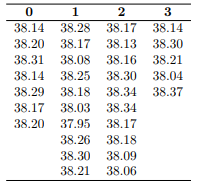
\includegraphics{table2.png}
\caption{}
\end{figure}

    \begin{Verbatim}[commandchars=\\\{\}]
{\color{incolor}In [{\color{incolor}54}]:} r \PY{o}{=} \PY{k+kt}{c}\PY{p}{(}\PY{l+m}{7}\PY{p}{,} \PY{l+m}{10}\PY{p}{,} \PY{l+m}{10}\PY{p}{,} \PY{l+m}{5}\PY{p}{)}
         types \PY{o}{=} \PY{k+kt}{c}\PY{p}{(}\PY{l+m}{0}\PY{p}{,} \PY{l+m}{1}\PY{p}{,} \PY{l+m}{2}\PY{p}{,} \PY{l+m}{3}\PY{p}{)}
         button\PYZus{}pushes\PYZus{}type \PY{o}{=} \PY{k+kp}{as.factor}\PY{p}{(}\PY{k+kt}{c}\PY{p}{(}\PY{k+kp}{rep}\PY{p}{(}types\PY{p}{[}\PY{l+m}{1}\PY{p}{]}\PY{p}{,} r\PY{p}{[}\PY{l+m}{1}\PY{p}{]}\PY{p}{)}\PY{p}{,}
                                 \PY{k+kp}{rep}\PY{p}{(}types\PY{p}{[}\PY{l+m}{2}\PY{p}{]}\PY{p}{,} r\PY{p}{[}\PY{l+m}{2}\PY{p}{]}\PY{p}{)}\PY{p}{,}
                                 \PY{k+kp}{rep}\PY{p}{(}types\PY{p}{[}\PY{l+m}{3}\PY{p}{]}\PY{p}{,} r\PY{p}{[}\PY{l+m}{3}\PY{p}{]}\PY{p}{)}\PY{p}{,}
                                 \PY{k+kp}{rep}\PY{p}{(}types\PY{p}{[}\PY{l+m}{4}\PY{p}{]}\PY{p}{,} r\PY{p}{[}\PY{l+m}{4}\PY{p}{]}\PY{p}{)}\PY{p}{)}\PY{p}{)}
         waiting\PYZus{}time \PY{o}{=} \PY{k+kt}{c}\PY{p}{(}\PY{l+m}{38.14}\PY{p}{,} \PY{l+m}{38.20}\PY{p}{,} \PY{l+m}{38.31}\PY{p}{,} \PY{l+m}{38.14}\PY{p}{,} \PY{l+m}{38.29}\PY{p}{,} \PY{l+m}{38.17}\PY{p}{,} \PY{l+m}{38.20}\PY{p}{,} 
                         \PY{l+m}{38.28}\PY{p}{,} \PY{l+m}{38.17}\PY{p}{,} \PY{l+m}{38.08}\PY{p}{,} \PY{l+m}{38.25}\PY{p}{,} \PY{l+m}{38.18}\PY{p}{,} \PY{l+m}{38.03}\PY{p}{,} \PY{l+m}{37.95}\PY{p}{,} \PY{l+m}{38.26}\PY{p}{,} \PY{l+m}{38.30}\PY{p}{,} \PY{l+m}{38.21}\PY{p}{,}
                         \PY{l+m}{38.17}\PY{p}{,} \PY{l+m}{38.13}\PY{p}{,} \PY{l+m}{38.16}\PY{p}{,} \PY{l+m}{38.30}\PY{p}{,} \PY{l+m}{38.34}\PY{p}{,} \PY{l+m}{38.34}\PY{p}{,} \PY{l+m}{38.17}\PY{p}{,} \PY{l+m}{38.18}\PY{p}{,} \PY{l+m}{38.09}\PY{p}{,} \PY{l+m}{38.06}\PY{p}{,}
                         \PY{l+m}{38.14}\PY{p}{,} \PY{l+m}{38.30}\PY{p}{,} \PY{l+m}{38.21}\PY{p}{,} \PY{l+m}{38.04}\PY{p}{,} \PY{l+m}{38.37}\PY{p}{)}
         pedestrian \PY{o}{=} \PY{k+kt}{data.frame}\PY{p}{(}button\PYZus{}pushes\PYZus{}type\PY{p}{,} waiting\PYZus{}time\PY{p}{)}
         pedestrian\PY{p}{[}\PY{k+kp}{sample}\PY{p}{(}\PY{k+kp}{nrow}\PY{p}{(}pedestrian\PY{p}{)}\PY{p}{,} \PY{l+m}{10}\PY{p}{)}\PY{p}{,} \PY{p}{]}
\end{Verbatim}

    \begin{tabular}{r|ll}
  & button\_pushes\_type & waiting\_time\\
\hline
	14 & 1     & 37.95\\
	11 & 1     & 38.25\\
	25 & 2     & 38.18\\
	27 & 2     & 38.06\\
	23 & 2     & 38.34\\
	2 & 0     & 38.20\\
	10 & 1     & 38.08\\
	17 & 1     & 38.21\\
	20 & 2     & 38.16\\
	13 & 1     & 38.03\\
\end{tabular}


    
    \begin{itemize}
\item
  \begin{enumerate}
  \def\labelenumi{(\alph{enumi})}
  \tightlist
  \item
    Plot the waiting times against the number of pushes of the button.
    What does the plot show?
  \end{enumerate}
\end{itemize}

    \begin{Verbatim}[commandchars=\\\{\}]
{\color{incolor}In [{\color{incolor}55}]:} \PY{k+kn}{library}\PY{p}{(}ggplot2\PY{p}{)}
         ggplot\PY{p}{(}pedestrian\PY{p}{,} aes\PY{p}{(}x\PY{o}{=}button\PYZus{}pushes\PYZus{}type\PY{p}{,} y\PY{o}{=}waiting\PYZus{}time\PY{p}{,} color\PY{o}{=}button\PYZus{}pushes\PYZus{}type\PY{p}{)}\PY{p}{)} \PY{o}{+}
                     geom\PYZus{}boxplot\PY{p}{(}\PY{p}{)} \PY{o}{+}
                     ylab\PY{p}{(}\PY{l+s}{\PYZsq{}}\PY{l+s}{waiting time\PYZsq{}}\PY{p}{)} \PY{o}{+}
                     ggtitle\PY{p}{(}\PY{l+s}{\PYZsq{}}\PY{l+s}{Boxplots of pedestrain waiting times\PYZsq{}}\PY{p}{)} \PY{o}{+}
                     theme\PY{p}{(}plot.title \PY{o}{=} element\PYZus{}text\PY{p}{(}hjust \PY{o}{=} \PY{l+m}{0.5}\PY{p}{)}\PY{p}{)} \PY{o}{+}
                     ylim\PY{p}{(}\PY{k+kp}{min}\PY{p}{(}pedestrian\PY{o}{\PYZdl{}}waiting\PYZus{}time\PY{p}{)}\PY{l+m}{\PYZhy{}0.2}\PY{p}{,} \PY{k+kp}{max}\PY{p}{(}pedestrian\PY{o}{\PYZdl{}}waiting\PYZus{}time\PY{p}{)}\PY{l+m}{+0.2}\PY{p}{)}
\end{Verbatim}

    
    
    \begin{center}
    \adjustimage{max size={0.7\linewidth}{0.7\paperheight}}{output_20_1.png}
    \end{center}
    { \hspace*{\fill} \\}
    
    \begin{itemize}
\tightlist
\item
  the mean of \(0, 1, 2, 3\) button pushes are quite similar to each
  other, stable at around 38.2, except for the mean of \(2\) pushes being
  slightly smaller;
\item
  the shortest waiting time falls in the group where \(pushes = 1\), the
  longest waiting time occurs when \(pushes = 3\);
\item
  the boxplots of these 3 button pushes share significant resemblance;
\end{itemize}

    \begin{itemize}
\item
  \begin{enumerate}
  \def\labelenumi{(\alph{enumi})}
  \setcounter{enumi}{1}
  \tightlist
  \item
    Write out the one-way ANOVA model for this experiment.
  \end{enumerate}
\end{itemize}

    \begin{Verbatim}[commandchars=\\\{\}]
{\color{incolor}In [{\color{incolor}56}]:} aov.pedestrian\PY{o}{=}aov\PY{p}{(}waiting\PYZus{}time\PY{o}{\PYZti{}}button\PYZus{}pushes\PYZus{}type\PY{p}{)}
         aov.pedestrian
\end{Verbatim}

    
    \begin{verbatim}
Call:
   aov(formula = waiting_time ~ button_pushes_type)

Terms:
                button_pushes_type  Residuals
Sum of Squares          0.00804714 0.30595286
Deg. of Freedom                  3         28

Residual standard error: 0.1045318
Estimated effects may be unbalanced
    \end{verbatim}

    
    \begin{itemize}
\item
  \begin{enumerate}
  \def\labelenumi{(\alph{enumi})}
  \setcounter{enumi}{2}
  \tightlist
  \item
    Use R to estimate the mean waiting time for each number of pushes.
  \end{enumerate}
\end{itemize}

    \begin{Verbatim}[commandchars=\\\{\}]
{\color{incolor}In [{\color{incolor}61}]:} lsm.pedestrian \PY{o}{=} lsmeans\PY{p}{(}aov.pedestrian\PY{p}{,} \PY{l+s}{\PYZsq{}}\PY{l+s}{button\PYZus{}pushes\PYZus{}type\PYZsq{}}\PY{p}{)}
         lsm.pedestrian
\end{Verbatim}

    
    \begin{verbatim}
 button_pushes_type   lsmean         SE df lower.CL upper.CL
 0                  38.20714 0.03950929 28 38.12621 38.28807
 1                  38.17100 0.03305584 28 38.10329 38.23871
 2                  38.19400 0.03305584 28 38.12629 38.26171
 3                  38.21200 0.04674802 28 38.11624 38.30776

Confidence level used: 0.95 
    \end{verbatim}

    
    \begin{itemize}
\item
  \begin{enumerate}
  \def\labelenumi{(\alph{enumi})}
  \setcounter{enumi}{3}
  \tightlist
  \item
    Show that the contrast \(\tau_1 - \tau_0\) is estimable, and use R
    to find it's LS estimate. This contrast compares the effect of no
    pushes of the button with the effect of pushing the button once.
  \end{enumerate}
\end{itemize}

    Suppose it is estimable, then it should be represented as

\[\tau_1- \tau_0 = b_0 (\mu + \tau_0) + b_1 (\mu + \tau_1) + b_2 (\mu + \tau_2) + b_3 (\mu + \tau_3)\]

\[= \mu (b_0+b_1+b_2+b_3) +  b_0 \tau_0 + b_1 \tau_1 + b_2 \tau_2 + b_3 \tau_3\]

\begin{align}
\left\{\begin{matrix} (b_0 + b_1+b_2+b_3) =0
\\ b_0 = -1
\\ b_1 = 1
\\ b_2 = 0
\\ b_3 = 0
\end{matrix}\right.
\end{align}

Therefore,
\(\tau_1- \tau_2 = (-1) \cdot (\mu + \tau_0) + 1 \cdot (\mu + \tau_1) + 0 \cdot (\mu + \tau_2) + 0 \cdot (\mu + \tau_3)\),
it is estimable.

    \begin{Verbatim}[commandchars=\\\{\}]
{\color{incolor}In [{\color{incolor}63}]:} contrast\PY{p}{(}lsm.pedestrian\PY{p}{,}\PY{k+kt}{list}\PY{p}{(}\PY{l+s}{\PYZdq{}}\PY{l+s}{1.minus.0\PYZdq{}}\PY{o}{=}\PY{k+kt}{c}\PY{p}{(}\PY{l+m}{\PYZhy{}1}\PY{p}{,} \PY{l+m}{1}\PY{p}{,} \PY{l+m}{0}\PY{p}{,} \PY{l+m}{0}\PY{p}{)}\PY{p}{)}\PY{p}{)}
\end{Verbatim}

    
    \begin{verbatim}
 contrast     estimate         SE df t.ratio p.value
 1.minus.0 -0.03614286 0.05151381 28  -0.702  0.4887

    \end{verbatim}

    
    \begin{itemize}
\item
  \begin{enumerate}
  \def\labelenumi{(\alph{enumi})}
  \setcounter{enumi}{4}
  \tightlist
  \item
    Show that the contrast \((\tau_1 + \tau_2 + \tau_3)/3 − \tau_0\) is
    estimable, and use R to find it's LS estimate. This contrast
    compares the effect of no pushes of the button with the effect of
    pushing the button at least once.
  \end{enumerate}
\end{itemize}

    Suppose it is estimable, then it should be represented as

\[(\tau_1 + \tau_2 + \tau_3)/3 - \tau_0 = b_0 (\mu + \tau_0) + b_1 (\mu + \tau_1) + b_2 (\mu + \tau_2) + b_3 (\mu + \tau_3)\]

\[= \mu (b_0+b_1+b_2+b_3) +  b_0 \tau_0 + b_1 \tau_1 + b_2 \tau_2 + b_3 \tau_3\]

\begin{align}
\left\{\begin{matrix} (b_0 + b_1+b_2+b_3) =0
\\ b_0 = -1
\\ b_1 = \frac{1}{3}
\\ b_2 = \frac{1}{3}
\\ b_3 = \frac{1}{3}
\end{matrix}\right.
\end{align}

Therefore,
\((\tau_1 + \tau_2 + \tau_3)/3 - \tau_0 = (-1) \cdot (\mu + \tau_0) + \frac{1}{3} \cdot (\mu + \tau_1) + \frac{1}{3} \cdot (\mu + \tau_2) + \frac{1}{3} \cdot (\mu + \tau_3)\),
it is estimable.


    
    \begin{Verbatim}[commandchars=\\\{\}]
{\color{incolor}In [{\color{incolor}66}]:} contrast\PY{p}{(}lsm.pedestrian\PY{p}{,}\PY{k+kt}{list}\PY{p}{(}\PY{l+s}{\PYZdq{}}\PY{l+s}{(1+2+3)/3.minus.0\PYZdq{}}\PY{o}{=}\PY{k+kt}{c}\PY{p}{(}\PY{l+m}{\PYZhy{}1}\PY{p}{,} \PY{l+m}{1}\PY{o}{/}\PY{l+m}{3}\PY{p}{,} \PY{l+m}{1}\PY{o}{/}\PY{l+m}{3}\PY{p}{,} \PY{l+m}{1}\PY{o}{/}\PY{l+m}{3}\PY{p}{)}\PY{p}{)}\PY{p}{)}
\end{Verbatim}

    
    \begin{verbatim}
 contrast             estimate         SE df t.ratio p.value
 (1+2+3)/3.minus.0 -0.01480952 0.04523962 28  -0.327  0.7458

    \end{verbatim}

    

    % Add a bibliography block to the postdoc
    
    
    
    \end{document}
